\subsection{Варианты использования}
	\subsubsection{Создать задание}
	\begin{enumerate}
		\item 	Пользователь авторизуется и выбирает кнопку <<создать задание>>
		\item 	Система отображает окно <<Новое задание>>
		\item 	Пользователь вводит описание задания и нажимает кнопку <<ОК>>
		\item 	Система уведомляет об успешном добавлении задания
	\end{enumerate}
	
	\textbf{\textit{Альтернатива: этап 1}} Пользователя с таким логином/паролем не существует: система выдает уведомление и просит ввести еще раз
	
	\subsubsection{Просмотреть список задач (работник)}
	\begin{enumerate}
		\item	Работник авторизуется
		\item	Система показывает список заданий, на которые он назначен, в порядке убывания приоритета		
	\end{enumerate}
		\textbf{\textit{Альтернатива: этап 1}} Работника с таким логином/паролем не существует: система выдает уведомление и просит ввести еще раз
			
	\subsubsection{Просмотреть список задач работника и снять задачу (менеджер)}
		\begin{enumerate}
		\item	Менеджер авторизуется
		\item	Менеджер выбирает работника из списка
		\item	Система показывает список задач, закрепленных за работником
		\item	Менеджер выбирает задачу и нажимает кнопку <<снять>>
		\item	Система убирает задачу из списка закрепленных за работником		
		\end{enumerate}
		
		\textbf{\textit{Альтернатива: Этап 1}} Менеджера с таким логином/паролем не существует: система выдает уведомление и просит ввести еще раз
		
	
	\subsubsection{Удалить задачу (менеджер)}
		\begin{enumerate}
		\item	Менеджер авторизуется
		\item	Менеджер выбирает работника из списка
		\item	Система показывает список задач, закрепленных за работником
		\item	Менеджер выбирает задачу и нажимает кнопку <<Удалить>>
		\item	Система удаляет задачу
		\end{enumerate}
		
		\textbf{\textit{Альтернатива: Этап 1}} Менеджера с таким логином/паролем не существует: система выдает уведомление и просит ввести еще раз
		
		\textbf{\textit{Альтернатива: Этап 2}} Менеджер выбирает свободную задачу и нажимает кнопку <<Удалить>>
		
	\subsubsection{Назначить задание работнику}
		\begin{enumerate}
		\item	Менеджер авторизуется
		\item	Система показывает список свободных задач
		\item	Менеджер выбирает задачу и нажимает кнопку <<Назначить>>
		\item	Система показывает окно <<Назначение задачи>> со списком работников и полем назначения приоритета
		\item	Менеджер выбирает работника и приоритет, нажимает кнопку <<ОК>>
		\item	Система уведомляет об успехе процедуры 			
		\end{enumerate}
		
		\textbf{\textit{Альтернатива: Этап 1}} Менеджера с таким логином/паролем не существует: система выдает уведомление и просит ввести еще раз
		
	\subsubsection{Пометить задание, как выполненное (работник)}
		\begin{enumerate}
		\item	Работник авторизуется
		\item	Система показывает список заданий, на которые он назначен, в порядке убывания приоритета
		\item	Работник выбирает задание и нажимает кнопку <<Задача готова>>
		\item	Система уведомляет об успехе операции				
		\end{enumerate}
	
		\textbf{\textit{Альтернатива: Этап 1}} Работника с таким логином/паролем не существует: система выдает уведомление и просит ввести еще раз
		
	\subsubsection{Пометить задание, как выполненное (менеджер)}
		\begin{enumerate}
			\item	Менеджер авторизуется
			\item	Менеджер выбирает работника из списка
			\item	Система показывает список задач, закрепленных за работником
			\item	Менеджер выбирает задачу и нажимает кнопку <<Задача готова>>						
		\end{enumerate}
		
		\textbf{\textit{Альтернатива: Этап 1}} Менеджера с таким логином/паролем не существует: система выдает уведомление и просит ввести еще раз
		
		\textbf{\textit{Альтернатива: Этап 2}} Менеджер выбирает свободную задачу и нажимает кнопку <<Задача готова>>
		
\subsection{Модель предметной области}
	\begin{figure}[H]
		\centering
		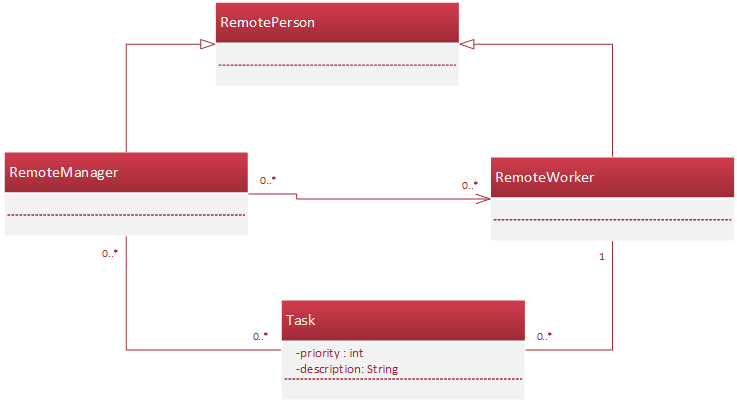
\includegraphics[width=1\textwidth]{../materials/EPDiagram.png}
		\caption{Модель предметной области}
		\label{fig:class_ob}
		\end{figure}